\newcommand{\saml}{SAML \emoji{old-man-dark-skin-tone}}

\chapter{SAML}

\begin{figure}[H]
      \centering
      
\includegraphics[width=8cm, keepaspectratio]{capitoli/id_managing/imgs/samuel.jpg}
      \caption{Diagramma riassuntivo di SAML 2.0.}
\end{figure}

Il \textit{Security Assertion Markup Language} (\textbf{SAML}) \emoji{old-man-dark-skin-tone} 2.0 fornisce due
funzioni molto importanti: \textit{Cross-domain Single Sign-On} (\textbf{SSO}) e
l'\textit{Identity Federation}. Questo è largamente utilizzato in ambito aziendale
in quanto permette di avere applicazioni che delegano l'autenticazione degli impiegati,
clienti e partner ad un identity provider centralizzato nell'azienda.\\

Il caso d'uso più comune per \saml{} 2.0 è la Cross-domain single sign-on (SSO) in cui
un utente ha la necessità di accedere a molteplici applicazioni che risiedono in
domini differenti (e.g.: application1.com, application2.com, ecc.).
Senza SSO l'utente avrebbe dovuto creare un account per ognuna di queste applicazioni
e loggarsi su ognuna individualmente, il che si traduce in molte credenziali che
l'utente deve ricordarsi e tenere al sicuro. Per un'azienda questo potrebbe essere
un problema molto importante in quanto dovrebbe trovarsi a gestire un grandissimo
numero di account. \saml{} permette alle applicazioni di delegare la fase dell'autenticazione
dell'utente ad un'entità remota chiamata Identity Provider.
Questa identità autentica l'utente e ritorna all'applicazione informazioni riguardanti
l'utente autenticato e la fase di autenticazione. Se l'utente accede ad una seconda
applicazione che delega l'autenticazione allo stesso Identity Provider,
non gli verrà richiesto di effettuare nuovamente il login ma potrà utilizzare
immediatamente il servizio.
\saml{} offre anche un altro meccanismo, chiamato Federated Identity, che permette
alle applicazioni e all'identity provider di utilizzare un unico identificatore
condiviso per un utente in modo da scambiare informazioni riguardo questo.

\section{Terminologia}

\saml{} definisce i seguenti termini:

\begin{itemize}
      \item \textbf{Subject}: un entità le cui informazioni verranno scambiate.
            Generalmente si riferisce a una persona che deve autenticarsi,
            ma può anche essere
            del software. In generale è un'entità in grado di autenticarsi.
      \item \textbf{SAML Assertion}: un messaggio sotto forma XML che contiene
            informazioni sulla sicurezza riguardo un subject.
      \item \textbf{SAML Profile}: un'insieme di regole di come usare i messaggi \saml{}
            per un business use case (come cross-domain single sign-on).
      \item \textbf{Identity Provider}: un ruolo definito per il profilo \saml{} di SSO.
            È un server che invia \saml{} Assertion riguardo un authenticated subject, nel
            contesto di SSO.
      \item \textbf{Service Provider}: un altro ruolo definito per il profilo \saml{} di
            SSO. Un service provider delega la fase di autenticazione ad un Identity
            Provider e si affida alle informazioni relative ad un authenticated
            subject ricevute dall'identity provider.
      \item \textbf{Trust Relationship}: un accordo tra un \saml{} Service Provider e un
            \saml{} Identity Provider dove il Service Provider si fida delle informazioni
            ricevute dall'Identity Provider.
      \item \textbf{SAML Protocol Binding}: una descrizione di come gli elementi
            dei messaggi \saml{} sono mappati in protocolli di comunicazione standard,
            come HTTP, per trasmetter informazioni tra il Service Provider e l'Identity
            Provider. In pratica, le richieste e risposte \saml{} sono inviate utilizzando
            il protocollo HTTPS tramite HTTP-Redirect o HTTP-POST, usando i relativi
            bindings, HTTP-Redirect Binding e HTTP-POST binding.
\end{itemize}

\section{Come Funziona ?}

L'utilizzo più comune di \saml{} è quello del Cross-domain web single sign-on.
In questo scenario l'utente che vuole utilizzare l'applicazione richiede l'autenticazione
all'applicazione (che opera come un \saml{} Service Provider). Questa poi delega la
richiesta al \saml{} Identity Provider che potrebbe anche trovarsi in un diverso
security domain. L'Identity Provider autentica l'utente e ritorna all'applicazione
un Security Token conosciuto come \saml{} Assertion. Questo token fornisce informazioni
sull'evento di autenticazione e sul soggetto autenticato. Affinché  venga implementata
l'abilità di effettuare il Cross-domain Web Single sign-on l'organizzazione che possiede
l'applicazione e l'identity provider scambia delle informazioni chiamate meta-dati
che contengono dati come gli \textit{URL endpoint} e i \textit{Certificati}
con cui validare i messaggi firmati digitalmente. Grazie a questi dati le due parti
possono scambiarsi messaggi poiché, grazie ai meta-dati, è possibile configurare
una relazione di fiducia tra il Service Provider e l'Identity Provider, questo è
necessario che avvenga affinché l'Identity Provider possa autenticare un utente
per il Service Provider. Una volta che questa configurazione mutuale dei provider
è impostata, quando un utente prova ad accedere al Server Provider, il suo
browser viene indirizzato all'identity provider con un \saml{} Authentication Request
Message. L'Identity Provider autenticherà l'utente per poi reindirizzarlo
all'applicazione con un \saml{} Authentication Response Message. Questa risposta
contiene una \saml{} Assertion con informazioni riguardo l'utente e l'evento di
autenticazione o di eventuali errori. L'Identity Provider può inserire le informazioni
che ritiene necessarie per il Service Provider in questione
all'interno dell'Assertion.

\subsection{SP-Initiated SSO}

\begin{figure}[H]
      \centering
      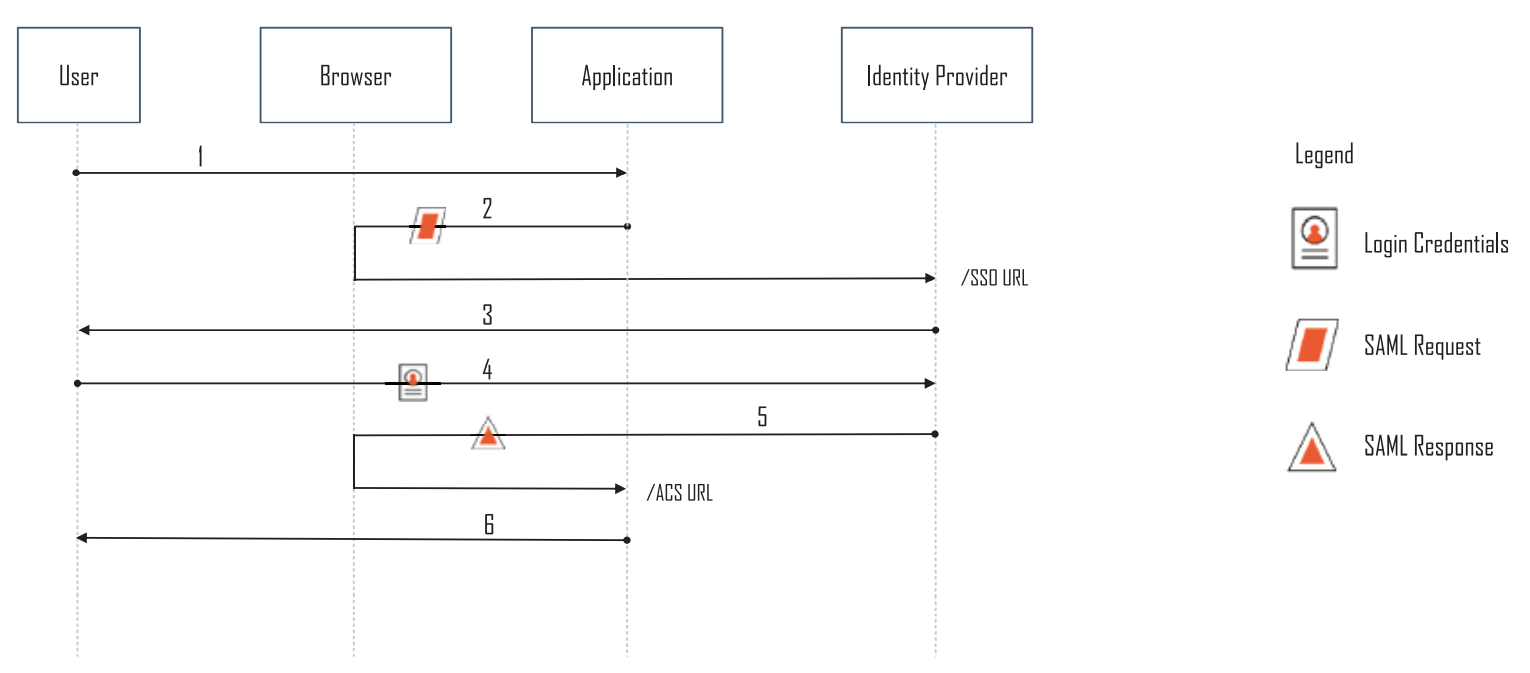
\includegraphics[width=\textwidth, keepaspectratio]{capitoli/id_managing/imgs/spsso.png}
\end{figure}

\begin{enumerate}
      \item L'utente visita un Service Provider.
      \item Il Service Provider reindirizza il browser dell'utente all'Identity
            Provider con una \saml{} Authentication Request.
      \item L'Identity Provider interagisce con l'utente per l'autenticazione.
      \item L'utente si autentica e l'Identity Provider valida le credenziali.
      \item L'Identity Provider reindirizza il browser dell'utente al
            Service Provider con una \saml{} Response che contiene a sua volta un \saml{}
            Authentication Assertion. La risposta è mandata
            all'\textit{Assertion Consumer Service}
            (ACS) URL del Service Provider.
      \item Il Service Provider consuma e valida la \saml{} Response e risponde alla
            richiesta originale dell'utente.
\end{enumerate}

\subsection{IdP-Initiated Flow}

A differenza dell'SP-Initiated Flow, l'IdP-Initiated Flow non parte dall'applicazione
ma direttamente dall'Identity Provider. Un implementazione di questo tipo può essere
vista in ambienti corporativi dove l'utente prima deve accedere al portale della
corporazione per poi poter utilizzare le varie applicazioni.
Un esempio è Office 365 che richiede
l'accesso con l'email dell'ateneo prima di poter utilizzare tutte
le sue funzionalità. In aggiunta, riduce il rischio che l'utente subisca un attacco
di phishing poiché si assicura che ogni applicazione abbia il corretto URL.

\begin{figure}[H]
      \centering
      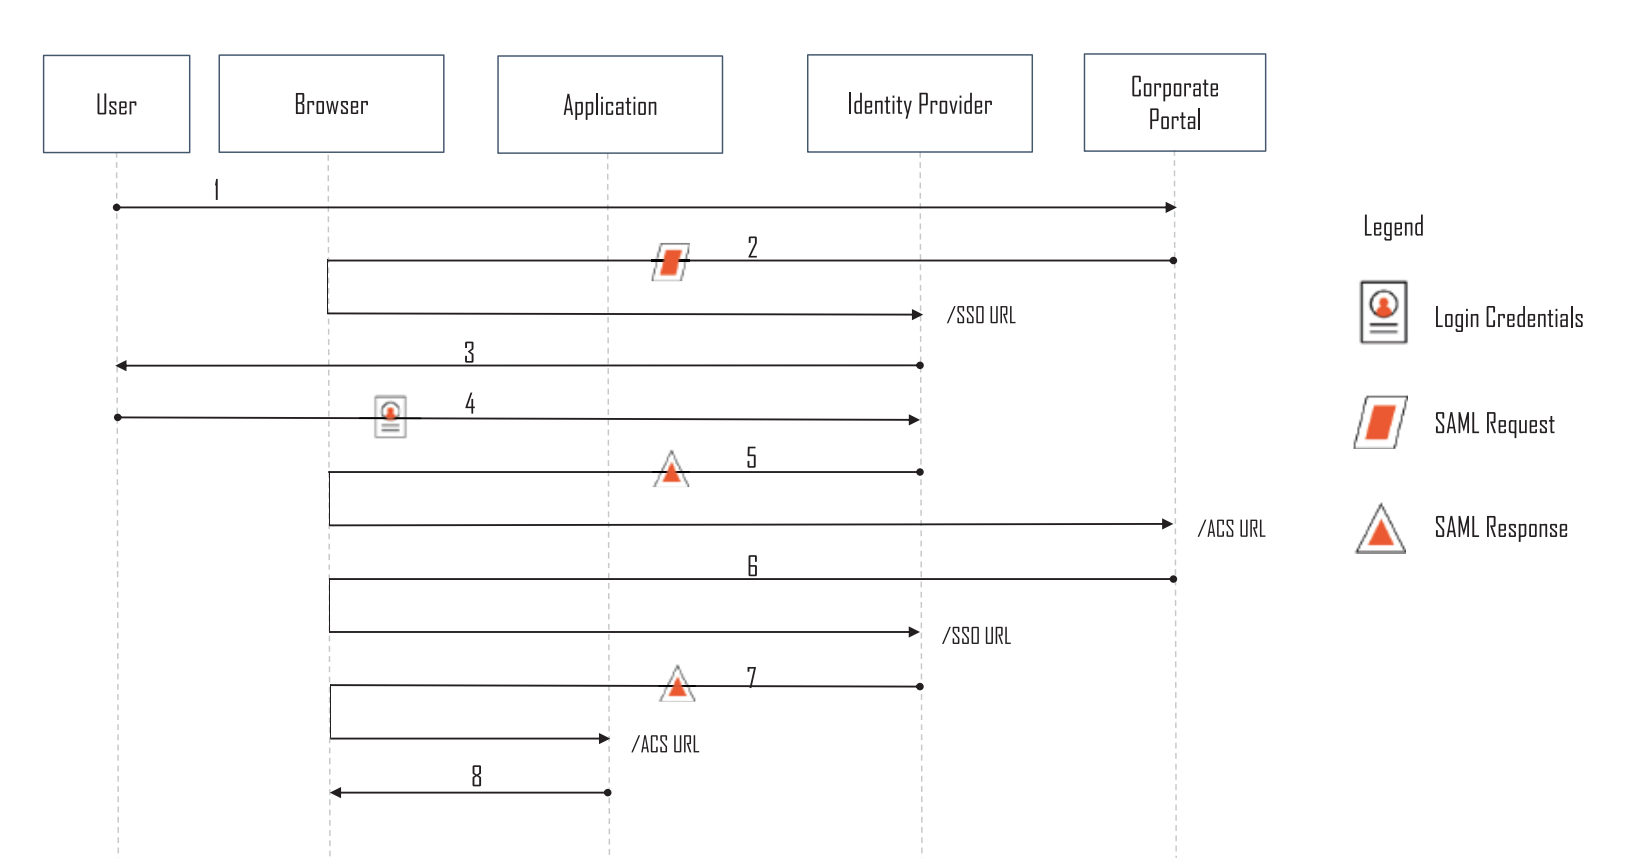
\includegraphics[width=\textwidth, keepaspectratio]{capitoli/id_managing/imgs/idp.png}
\end{figure}

\begin{enumerate}
      \item L'utente visita il portale della corporazione.
      \item Il portare reindirizza l'utente all'Identity Provider con una \saml{}
            Authentication Request.
      \item L'Identity Provider interagisce con l'utente per l'autenticazione.
      \item L'utente si autentica e l'Identity Provider valida le credenziali.
      \item L'Identity Provider reindirizza il browser dell'utente al portale con
            una \saml{} Response che contiene un'Authentication Assertion. L'utente
            viene autenticato nel portale che mostra i suoi contenuti all'utente
            inclusa una lista delle applicazioni.
      \item L'utente clicca un link nel portale per un'applicazione. Il link
            indirizza l'utente all'Identity Provider con un parametro che indica
            l'applicazione avviata. L'Identity Provider controlla la sessione
            dell'utente che nel diagramma mostrato sopra risulta sempre valida.
      \item L'Identity Provider reindirizza il browser dell'utente al URL Assertion
            Consumer Service del Service Provider con un nuova \saml{} Response per
            quell'applicazione.
      \item L'applicazione consuma la \saml{} Response e l'Authentication Assertion ed
            effettua il rendering della pagina appropriata per l'utente.
\end{enumerate}

\section{Identity Federation}

Con \saml{} è necessario che ci sia un'identificatore di comune accordo tra
l'Identity Provider ed il Service Provider che permetta di identificare l'utente.
Questo viene deciso quando gli amministratori del Service Provider scambiano
meta-dati riguardo i loro ambienti e li utilizzano per creare
la \textit{Federation Information} tra la loro applicazione e l'Identity Provider.
L'Identity Provider dovrà poi essere in gradi di fornire i corretti dati relativi
ad ogni potenziale Service Provider.

\begin{figure}[H]
      \centering
      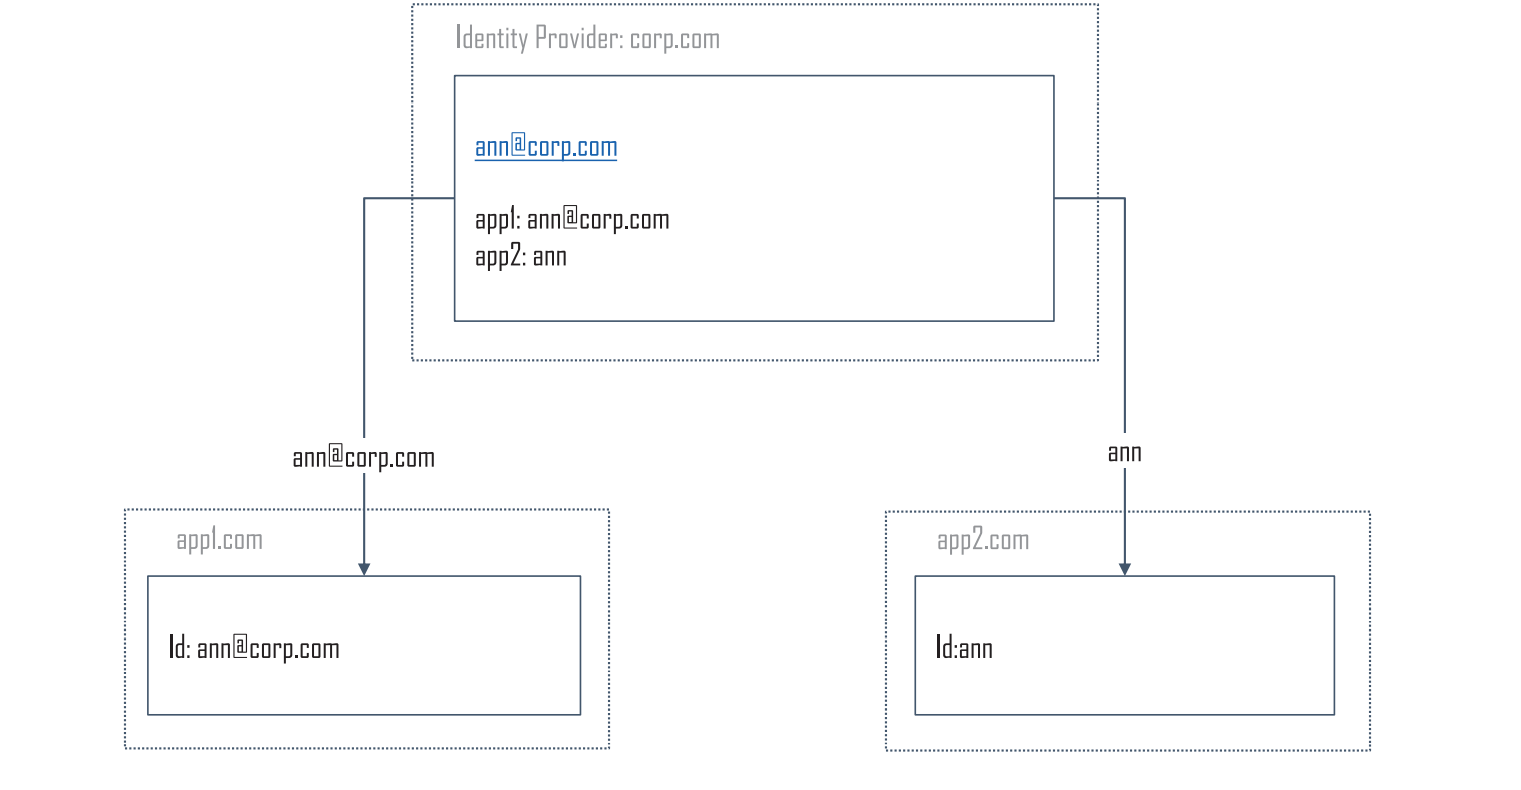
\includegraphics[width=\textwidth, keepaspectratio]{capitoli/id_managing/imgs/federation.png}
\end{figure}

\section{Authentication Brokers}

L'implementazione di \saml{} spesso risulta essere molto costosa e complessa dunque
per facilitarla invece che implementarlo direttamente sulla propria applicazione
si può utilizzare un \textit{Authentication Broker} che ci permette
di implementare
un protocollo di identità più nuovo, come OIDC, consentendo comunque la
comunicazione con un Identity Provider tramite dei protocolli.

\begin{figure}[H]
      \centering
      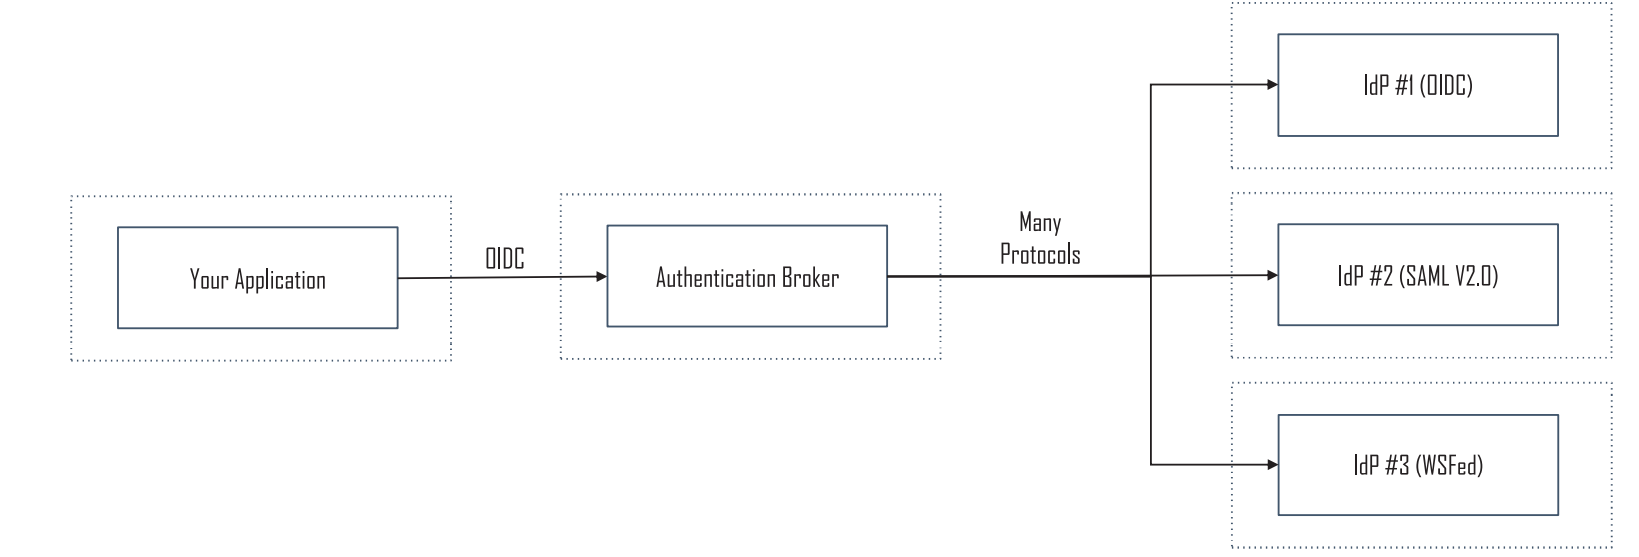
\includegraphics[width=\textwidth, keepaspectratio]{capitoli/id_managing/imgs/broker.png}
\end{figure}

\section{Benefici di SAML}

\begin{itemize}
      \item \textbf{Usability}: accesso One-Click da portali o intranet, password
            elimination, deep linking e rinnovamento automatico della sessione
            rendono la vita dell'utente molto più facile.
      \item \textbf{Security}: basato su forti firme digitali per l'autenticazione
            e l'integrità, \saml{} risulta essere un protocollo sicuro.
      \item \textbf{Speed}: \saml{} è veloce \footnote{Per ogni dubbio visionare \url{https://www.youtube.com/watch?v=BrP0H-n0x3Q}}.
      \item \textbf{Phishing Prevention}: se non hai una password per l'app non
            verrai ingannato per entrare in una fake login page.
      \item \textbf{IT Friendly}: \saml{} semplifica la vita per IT perché centralizza
            l'autenticazione, fornisce grande visibilità e render la
            directory integration
            più facile.
\end{itemize}